\section{Results}
\label{sec:results}

This section presents the empirical results obtained from evaluating the Large Language Models, \texttt{llama3.1} and \texttt{phi4}, on the dynamic benchmark suite we have developed and derived from the \emph{Logical Foundations} dataset. 
The core of the evaluation lies in comparing the models' ability to generate compilable Coq proofs for original theorems versus their semantically equivalent, identifier-renamed (mutated) counterparts. 
Success is primarily measured by whether the Coq compiler (\texttt{coqc}) accepted the LLM-generated proof. 
We also tracked instances where the LLM output was deemed unusable prior to compilation (termed "failures").

\noindent Overall, it is worth noting the following major points:
\begin{itemize}
  \item The \textbf{models tested were not fine-tuned to Coq or theorem proving tasks}, and the results reflect their performance in a zero-shot setting.
  \item The models were \textbf{run in a limited hardware environment}, and thus had to be run on smaller model sizes.
  \item \textbf{Theorem proving is a challenging task for LLMs.} The models struggled to produce compilable proofs, even for original theorems. See Section~\ref{sec:related-work} for a discussion of the state of the art in LLMs for theorem proving.
\end{itemize}

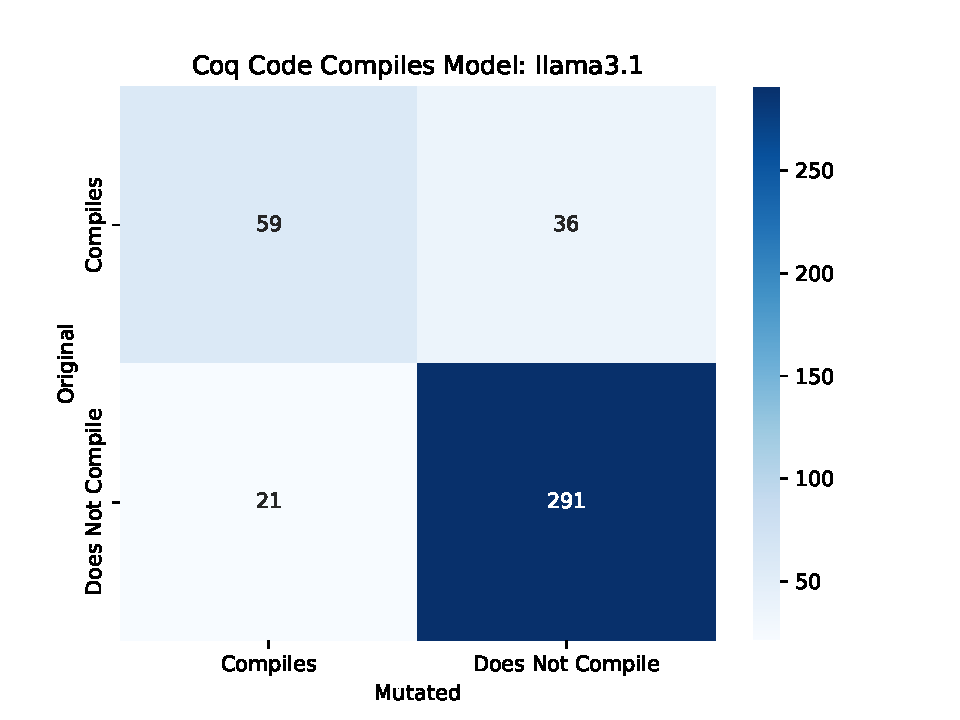
\includegraphics[width=0.50\textwidth]{CM_Compiles_Model_llama3.1}
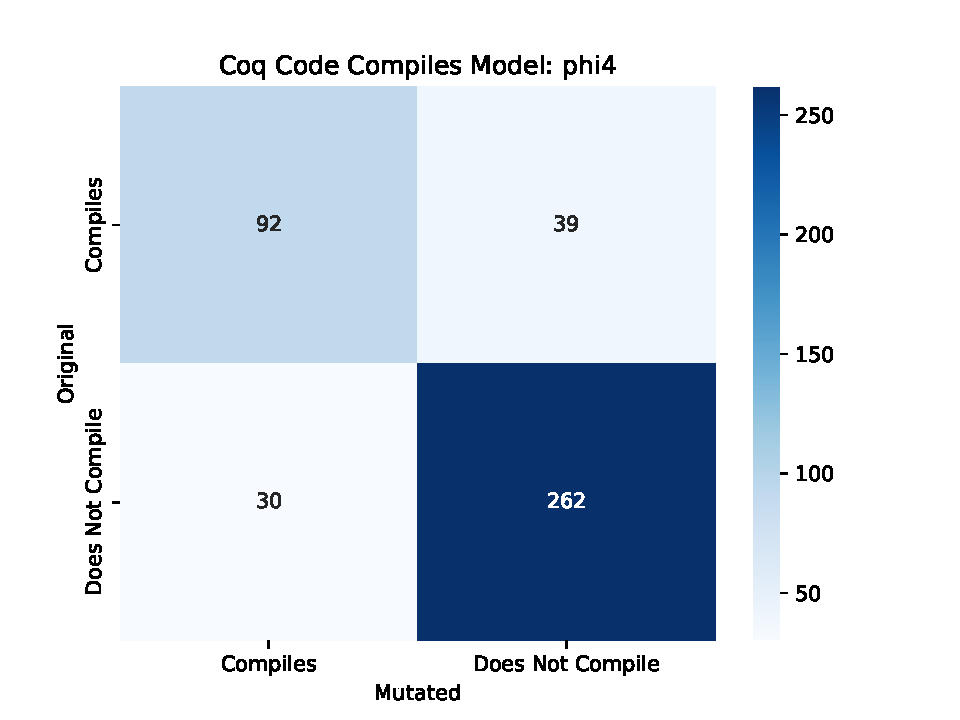
\includegraphics[width=0.50\textwidth]{CM_Compiles_Model_phi4}

\subsection{Overall Performance Statistics}
\label{sec:results_overall}

Across both models and both conditions (original and mutated), a total of 212 unique theorems from \emph{Logical Foundations} were used. Each theorem was presented to each model in its original and mutated form, leading to $212 \times 2 = 424$ theorem-proving attempts per model, or $828$ total attempts across the experiment. Table~\ref{tab:overall-stats} summarizes the aggregate performance.

\begin{table}[h]
\centering
\begin{tabular}{| p{4.5cm} | >{\raggedleft\arraybackslash}b{3cm} |}
\hline
\textbf{Metric} & \textbf{Value} \\
\hline
Total entries & 848 \\
Total Original Compiles & 226 (26.65\%) \\
Total Original Failed & 15 (1.77\%) \\
Total Mutated Compiles & 207 (24.41\%) \\
Total Mutated Failed & 3 (0.35\%) \\
\hline
\end{tabular}
\caption{Overall basic statistics across all models. ``Total entries'' refers to the total number of original or mutated theorem attempts (424 per model) across both models.}
\label{tab:overall-stats}
\end{table}

As indicated in Table~\ref{tab:overall-stats}, when pooling results from both \texttt{llama3.1} and \texttt{phi4}, the success rate for generating compilable proofs for original theorems was 26.65\% (226 out of 848 total original attempts). This rate decreased to 24.41\% (207 out of 848 total mutated attempts) for the mutated versions of the same theorems. This overall trend suggests that the identifier renaming impacted the models' ability to produce correct proofs.
Interestingly, the rate of pre-compilation failures (outputs deemed unusable before attempting compilation) was low overall, and \textbf{slightly lower for mutated theorems (0.35\%) compared to original theorems (1.77\%)}. This counter-intuitive result may suggest that the models were more likely to produce syntactically valid outputs when faced with the renamed identifiers, even if those outputs were not logically correct.

\subsection{Model-Specific Performance}
\label{sec:results_model_specific}

Tables~\ref{tab:kpi-percentages} (compilation and failure rates as percentages) and~\ref{tab:kpi-counts} (absolute counts) provide a detailed breakdown of performance for each model on the 424 unique theorems.

% User-provided Table 1 (KPI Percentages) - included here for context in the text
\begin{table}[h]
\centering
\begin{tabular}{|l|r|r|r|r|r|}
\hline
\textbf{Model} & \textbf{Entries} & \textbf{Orig. Compile \%} & \textbf{Mut. Compile \%} & \textbf{Orig. Fail \%} & \textbf{Mut. Fail \%} \\
\hline
llama3.1 & 424 & 22.41 & 19.81 & 3.30 & 0.71 \\
llama3.1 (no failures) & 407& 23.34 & 19.66 & 0.00 & 0.00 \\
\hline
phi4 & 424 & 30.90 & 29.01 & 0.24 & 0.00 \\
phi4 (no failures) & 423 & 30.97 & 28.84 & 0.00 & 0.00 \\
\hline
\end{tabular}
\caption{Compilation and failure rates by model (percentages). ``Entries'' refers to the number of unique theorems. For ``(no failures)'' rows, ``Entries'' refers to the subset of unique theorems where the model had no pre-compilation failures on either the original or mutated version.}
\label{tab:kpi-percentages}
\end{table}

% \begin{table}[h]
% \centering
% \begin{tabular}{|l|r|r|r|r|r|}
% \hline
% \textbf{Model} & \textbf{Entries} & \textbf{Orig. Compile} & \textbf{Mut. Compile} & \textbf{Orig. Fail} & \textbf{Mut. Fail} \\
% \hline
% llama3.1 & 424 & 95 & 84 & 14 & 3 \\
% llama3.1 (no failures) & 407 & 95 & 80 & 0 & 0 \\
% \hline
% phi4 & 424 & 131 & 123 & 1 & 0 \\
% phi4 (no failures) & 423 & 131 & 122 & 0 & 0 \\
% \hline
% \end{tabular}
% \caption{Compilation and failure outcomes by model (counts). ``Entries'' refers to the number of unique theorems.}
% \label{tab:kpi-counts}
% \end{table}

\subsubsection{Performance of \texttt{llama3.1}}
\label{sssec:results_llama31}
For \texttt{llama3.1}, the compilation success rate for original theorems was 22.41\% (95 out of 424 theorems), as detailed in Table~\ref{tab:kpi-percentages}. When presented with the mutated versions of these theorems, the success rate dropped to 19.81\% (84 theorems). This represents a decrease of 2.60 percentage points, or a relative reduction in performance of approximately 11.6\% ($ (22.41 - 19.81) / 22.41 \times 100\% $). The pre-compilation failure rate for \texttt{llama3.1} was 3.30\% (14 instances) for original theorems and 0.71\% (3 instances) for mutated theorems.

\subsubsection{Performance of \texttt{phi4}}
\label{sssec:results_phi4}
The \texttt{phi4} model demonstrated a \textbf{higher overall performance}. It successfully compiled proofs for 30.90\% of the original theorems (131 out of 424), according to Table~\ref{tab:kpi-percentages}. For the mutated theorems, this rate decreased to 29.01\% (123 theorems). This is a smaller decrease of 1.89 percentage points compared to \texttt{llama3.1}, corresponding to a relative performance reduction of approximately 6.1\% ($ (30.90 - 29.01) / 30.90 \times 100\% $). The pre-compilation failure rates for \texttt{phi4} were notably low: 0.24\% (1 instance) for original theorems and 0.00\% (0 instances) for mutated theorems.

\subsection{Results Discussion}
\label{sec:results_summary_observations}
The results indicate several key points:
\begin{itemize}
    \item Both \texttt{llama3.1} and \texttt{phi4} exhibited a measurable (albeit not significant) decrease in their ability to generate compilable Coq proofs when theorem identifiers were renamed, even though the logical structure and provability remained identical.
    \item \texttt{phi4} generally outperformed \texttt{llama3.1} in terms of overall proof compilation success rates on both original and mutated theorems.
    \item \texttt{phi4} also appeared slightly more robust to identifier mutations than \texttt{llama3.1}, showing a smaller relative decrease in performance.
    \item The persistence of the performance gap even when analyzing only ``no failure'' attempts suggests that the impact of renaming goes beyond merely causing issues with the generation of syntactically parsable output, affecting the subsequent logical correctness of the generated proofs.
    \item Pre-compilation failure rates were generally low and, somewhat counter-intuitively, lower for mutated theorems than for original ones.
\end{itemize}
These findings suggest that \textbf{current LLMs, to varying degrees, may rely on patterns associated with specific identifier names encountered during training, and that our dynamic benchmark approach is effective in revealing such sensitivities.}